\documentclass{article}

\usepackage{postprocess/context/arxiv}

\usepackage[utf8]{inputenc} % allow utf-8 input
\usepackage{amsmath}
\usepackage[T1]{fontenc}    % use 8-bit T1 fonts
\usepackage{hyperref}       % hyperlinks
\usepackage{url}            % simple URL typesetting
\usepackage{booktabs}       % professional-quality tables
\usepackage{amsfonts}       % blackboard math symbols
\usepackage{nicefrac}       % compact symbols for 1/2, etc.
\usepackage{microtype}      % microtypography
\usepackage{graphicx}
\usepackage{natbib}
\usepackage{doi}
\usepackage{float}
\usepackage{subcaption}
\usepackage{wrapfig}

\title{Causal Discovery Report on Abalone}

\author{ \href{https://orcid.org/0000-0000-0000-0000}{
\includegraphics[scale=0.06]{postprocess/context/orcid.pdf}\hspace{1mm}Causal Copilot}}

\renewcommand{\headeright}{Technical Report}
\renewcommand{\undertitle}{Technical Report}

\hypersetup{
pdftitle={Causal Discovery Report on Abalone},
pdfauthor={Causal Copilot},
pdfkeywords={Causal Discovery, Large Language Model, PC, Abalone},
}

\begin{document}
\maketitle

\begin{abstract}
This report presents a comprehensive causal discovery analysis of a dataset comprising various metrics associated with abalones, a marine mollusk species. We applied multiple causal discovery algorithms, including PC, GES, and NOTEARS, chosen for their suitability given the dataset's characteristics and sample size of 4,177. Our findings reveal significant causal relationships, such as the influence of Age on Diameter and Viscera weight, and the impact of Length on Shell and Shucked weights. Additionally, we implemented graph tuning techniques leveraging Bootstrap and expert insights from a large language model to refine the causal graph and enhance its robustness. The results provide valuable insights into the growth and development patterns of abalones, contributing to a deeper understanding of their biology and potential implications for commercial applications. However, discrepancies between statistical confidence and biological relevance suggest that further exploration is necessary to validate some causal connections.
\end{abstract}

\keywords{Causal Discovery, Large Language Model, PC, Abalone}

\raggedbottom
\section{Introduction}
The dataset under investigation encompasses a range of variables pertaining to abalones, a unique group of marine mollusks known for their ecological and commercial significance. Key metrics included are age, length, shell weight, diameter, height, whole weight, shucked weight, and viscera weight. Each of these variables provides critical insights into the growth patterns, health, and reproductive status of abalones, reflecting their complex biological and ecological interactions. The relationships among these variables are expected to exhibit causal patterns that can enhance our understanding of abalone development, influenced by factors such as environmental conditions, reproductive cycles, and commercial fishing practices. This report aims to apply causal discovery methodologies to elucidate these relationships, ultimately contributing to the knowledge base surrounding abalone biology and commerce.

\section{Background Knowledge}
\subsection{Detailed Explanation about the Variables}
The dataset contains various variables related to abalones, which are a type of marine mollusk. Each variable provides important insights into the characteristics and biology of abalones:

\begin{itemize}
\item \textbf{Age}: This variable represents the age of an abalone, expressed in years. Since abalones do not exhibit distinct physical age markers, age is often estimated through measurements of growth-related characteristics. Understanding the age of an abalone is crucial for assessing its development and reproductive potential.

\item \textbf{Length}: The length of the abalone is measured in millimeters along the longest dimension of its shell. Length serves as a key indicator of growth and overall health, impacting the abalone's competitive abilities in the environment and its vulnerability to predation.

\item \textbf{Shell Weight}: Measured in grams, this variable captures the weight of the abalone's shell. Shell weight is an important parameter that reflects both the health and maturity of the abalone, as heavier shells are typically associated with older and better-nourished individuals.

\item \textbf{Diameter}: The diameter of the abalone's shell, measured at its widest point in millimeters, is another metric that contributes to understanding its size and maturity. A larger diameter often correlates with a longer length and greater overall robustness of the abalone.

\item \textbf{Height}: This variable measures the height of the abalone's shell from the base to the apex in millimeters. Height can provide valuable information regarding the morphology and growth patterns of the abalone, which is essential when assessing its age and health.

\item \textbf{Whole Weight}: Represented in grams, whole weight refers to the total mass of the abalone, including the shell and all edible tissues. This measure is critical for evaluating the abalone's biomass and overall condition.

\item \textbf{Shucked Weight}: This variable denotes the mass of the abalone's edible portion after the shell has been removed, measured in grams. Shucked weight is particularly important in commercial contexts, where it directly relates to market value and culinary applications.

\item \textbf{Viscera Weight}: This weight refers to the mass of the internal organs of the abalone, measured in grams. Viscera weight can be indicative of the health and reproductive status of the organism, reflecting its condition and potential for spawning.
\end{itemize}

Each of these variables plays a vital role in understanding the biology, growth, and ecological dynamics of abalones. They are interconnected in ways that offer insights into causal relationships that can be explored further through causal discovery methods.

\subsection{Possible Causal Relations among these Variables}

\begin{minipage}[t]{0.7\linewidth}
\begin{itemize}
\item \textbf{Age $\rightarrow$ Length}: As abalones age, they typically increase in length due to continued growth, making age a key determinant of size.
\item \textbf{Age $\rightarrow$ Diameter}: The diameter of an abalone's shell often increases with age, as older abalones develop larger shells.
\item \textbf{Age $\rightarrow$ Height}: Height is influenced by age since older abalones generally have greater shell height as a result of growth over time.
\item \textbf{Length $\rightarrow$ Whole Weight}: An increase in length correlates with a higher whole weight, as larger abalones contain more soft tissue and shell.
\item \textbf{Length $\rightarrow$ Shell Weight}: Longer abalones tend to have heavier shells, as the shell weight increases with the size of the abalone.
\item \textbf{Length $\rightarrow$ Shucked Weight}: Greater length often leads to increased shucked weight, as longer abalones provide more edible tissue once the shell is removed.
\item \textbf{Length $\rightarrow$ Viscera Weight}: Longer abalones are likely to have higher viscera weight, as they contain more internal organs relative to their size.
\item \textbf{Diameter $\rightarrow$ Whole Weight}: An increase in diameter leads to a higher whole weight, as larger diameter abalones possess more biomass.
\item \textbf{Diameter $\rightarrow$ Shell Weight}: The shell's diameter is directly related to its weight, with larger diameters resulting in heavier shells.
\item \textbf{Diameter $\rightarrow$ Shucked Weight}: As the diameter increases, the shucked weight likely increases as well, due to more prominent soft tissue.
\item \textbf{Diameter $\rightarrow$ Viscera Weight}: A larger diameter can indicate a greater viscera weight, as bigger abalones may have more developed internal organs.
\item \textbf{Height $\rightarrow$ Whole Weight}: Height influences whole weight; taller abalones generally weigh more due to increased biomass.
\item \textbf{Height $\rightarrow$ Shell Weight}: Increased height correlates with shell weight, as taller shells typically have greater structural mass.
\item \textbf{Height $\rightarrow$ Shucked Weight}: Taller abalones are expected to have a higher shucked weight, as height may be associated with more edible tissue.
\item \textbf{Height $\rightarrow$ Viscera Weight}: Height can influence viscera weight, as larger abalones can potentially house more internal organs.
\item \textbf{Shell Weight $\rightarrow$ Whole Weight}: Heavier shells contribute significantly to the overall whole weight of the abalone.
\item \textbf{Whole Weight $\rightarrow$ Shucked Weight}: A larger whole weight is likely to result in a greater shucked weight, as it reflects the amount of soft tissue available post-harvest.
\item \textbf{Whole Weight $\rightarrow$ Viscera Weight}: Heavier whole weights generally indicate more fleshy and viscera mass, leading to increased viscera weight.
\item \textbf{Shucked Weight $\rightarrow$ Viscera Weight}: An increase in shucked weight may correlate with an increase in viscera weight, as more meat can imply a larger internal organ mass.
\end{itemize}
\fill
\end{minipage}
\hspace{0.05\textwidth}
\begin{minipage}[t]{0.3\linewidth}
    \begin{figure}[H]
        \centering
        \resizebox{\linewidth}{!}{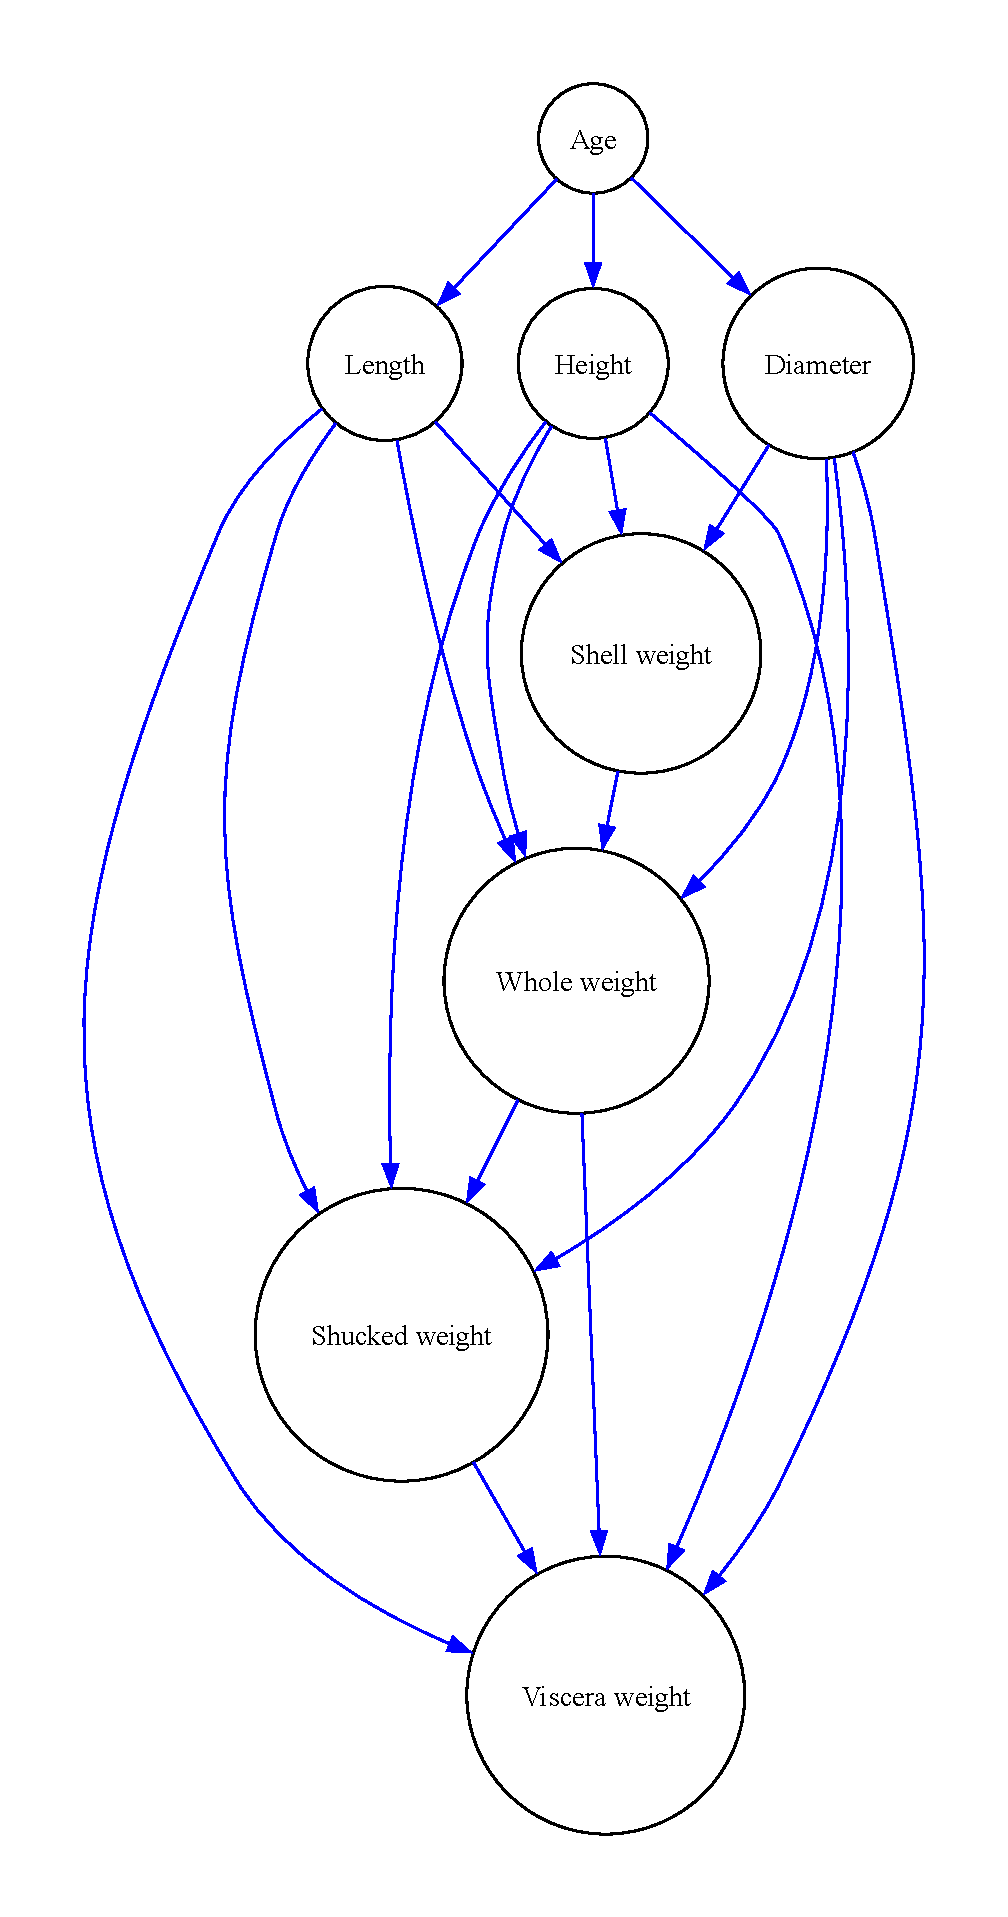
\includegraphics[height=0.4\textheight]{./demo_data/20241104_094220/Abalone/output_graph/potential_relation.pdf}}
        \caption{\label{fig:relation}Possible Causal Relation Graph}
    \end{figure}
\end{minipage}

\section{Dataset Descriptions and EDA}
The following is a preview of our original dataset.

\begin{table}[H]
    \centering
    \caption{Dataset Preview}
    \begin{tabular}{rrrrrrrr}
\toprule
 Age &  Length &  Shell weight &  Diameter &  Height &  Whole weight &  Shucked weight &  Viscera weight \\
\midrule
15.0 &   0.455 &         0.365 &     0.095 &  0.5140 &        0.2245 &          0.1010 &           0.150 \\
 7.0 &   0.350 &         0.265 &     0.090 &  0.2255 &        0.0995 &          0.0485 &           0.070 \\
 9.0 &   0.530 &         0.420 &     0.135 &  0.6770 &        0.2565 &          0.1415 &           0.210 \\
10.0 &   0.440 &         0.365 &     0.125 &  0.5160 &        0.2155 &          0.1140 &           0.155 \\
 7.0 &   0.330 &         0.255 &     0.080 &  0.2050 &        0.0895 &          0.0395 &           0.055 \\
\bottomrule
\end{tabular}
\end{table}

\subsection{Data Properties}
We employ several statistical methods to identify data properties.

The shape of the data, data types, and missing values are assessed directly from the dataframe.
Linearity is evaluated using Ramsey’s RESET test, followed by the Benjamini \& Yekutieli procedure for multiple test correction.
Gaussian noise is assessed through the Shapiro-Wilk test, also applying the Benjamini \& Yekutieli procedure for multiple test correction.
Time-Series and Heterogeneity are derived from user queries.

Properties of the dataset we analyzed are listed below.

\begin{table}[H]
    \centering
    \caption{Data Properties}

        \begin{tabular}{rrrrrrr}
        \toprule
            Shape ($n$ x $d$) & Data Type & Missing Value & Linearity & Gaussian Errors & Time-Series & Heterogeneity \\
            \midrule
            (4177, 8)   & Continuous & False & True & True & False & False \\
            \bottomrule
        \end{tabular}
\end{table}

\subsection{Distribution Analysis}
The following figure shows distributions of different variables. The orange dash line represents the mean, 
and the black line represents the median. Variables are categorized into three types according to their distribution characteristics.

\begin{figure}[H]
\centering
\includegraphics[width=\linewidth]{./demo_data/20241104_094220/Abalone/output_graph/eda_dist.jpg}
\caption{\label{fig:dist}Distribution Plots of Variables}
\end{figure}

\begin{itemize}
\item Slight left skew distributed variables: Length, Shell Weight, Diameter, Whole Weight
\item Slight right skew distributed variables: Age, Height, Shucked Weight, Viscera Weight
\item Symmetric distributed variables: None
\end{itemize}

\subsection{Correlation Analysis}

\begin{minipage}[t]{0.5\linewidth}
    In this analysis, we will categorize the correlation statistics of features in the dataset into three distinct categories: Strong correlations, Moderate correlations, and Weak correlations.

\begin{itemize}
\item Strong Correlated Variables: Shell weight and Length, Height and Whole weight, Shucked weight and Height, Viscera weight and Height, Viscera weight and Shell weight, Shucked weight and Shell weight, Viscera weight and Shucked weight
\item Moderate Correlated Variables: Length and Age, Shell weight and Age, Diameter and Age, Height and Age, Whole weight and Diameter, Shucked weight and Diameter, Whole weight and Height, Whole weight and Shucked weight, Diameter and Height
\item Weak Correlated Variables: Shucked weight and Age
\end{itemize}
\vfill
\end{minipage}
\hfill
\begin{minipage}[t]{0.5\linewidth}
    \begin{figure}[H]
        \centering
        \vspace{-1.5cm}
        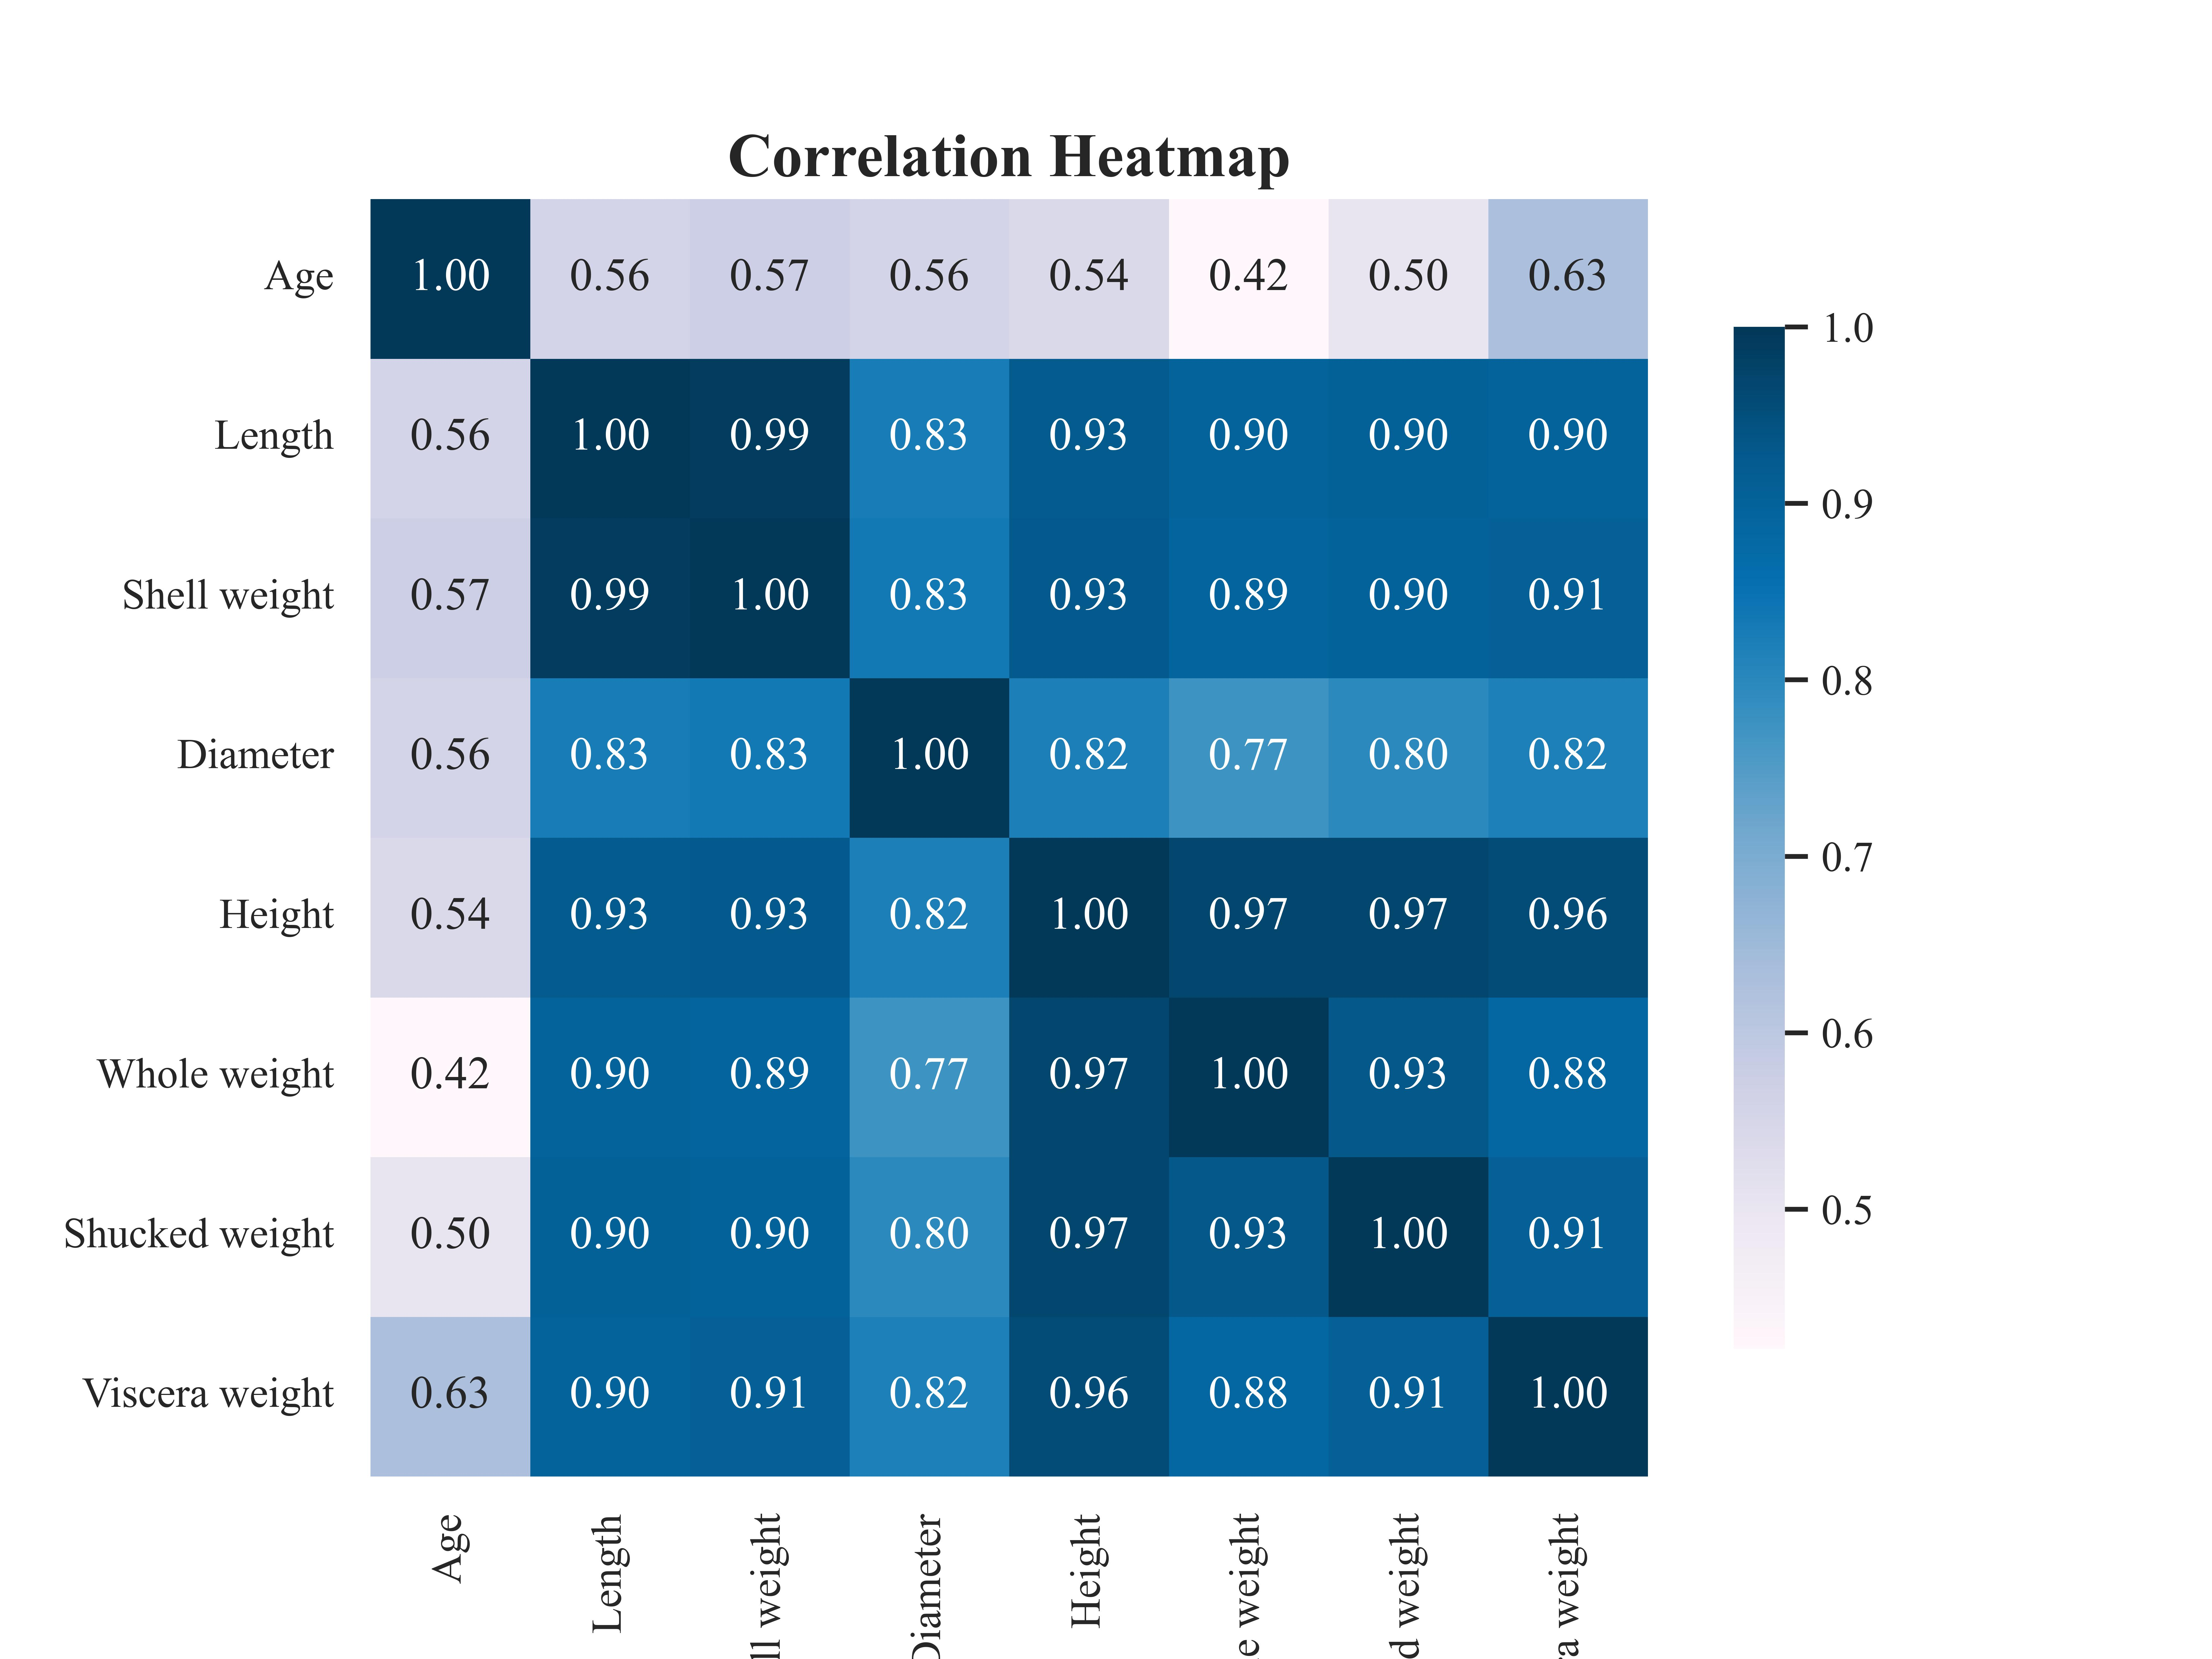
\includegraphics[width=\linewidth]{./demo_data/20241104_094220/Abalone/output_graph/eda_corr.jpg}
        \caption{\label{fig:corr}Correlation Heatmap of Variables}
    \end{figure}
\end{minipage}

\section{Discovery Procedure}

In this section, we provide a detailed description of the causal discovery process implemented by Causal Copilot. 
We also provide the chosen algorithms and hyperparameters, along with the justifications for these selections.

\subsection{Data Preprocessing}
In this initial step, we preprocessed the data and examined its statistical characteristics. 
This involved cleaning the data, handling missing values, and performing exploratory data analysis to understand distributions and relationships between variables.
                
\subsection{Algorithm Selection assisted with LLM}
Following data preprocessing, we employed a large language model (LLM) to assist in 
selecting appropriate algorithms for causal discovery based on the statistical characteristics of the dataset and relevant background knowledge. 
The top three chosen algorithms, listed in order of suitability, are as follows:   
        
\begin{itemize}

\item \textbf{PC}:
\begin{itemize}
    \item \textbf{Description}: The PC algorithm is a constraint-based method that learns the structure of a causal graph from data by testing conditional independencies between variables, resulting in a Directed Acyclic Graph (DAG).
    \item \textbf{Justification}: Given the large sample size of 4177 and the assumption that all relevant variables are observed with predominantly linear relationships, PC is efficient for large-scale data and provides a good balance between computational efficiency and the need for a causal structure.
\end{itemize}

\item \textbf{GES}:
\begin{itemize}
    \item \textbf{Description}: Greedy Equivalence Search (GES) is a score-based causal discovery algorithm that identifies the optimal causal structure by navigating the space of equivalence classes of Directed Acyclic Graphs (DAGs) using a scoring criterion like the Bayesian Information Criterion (BIC).
    \item \textbf{Justification}: GES is suitable due to the dataset's linear relationships and sufficient sample size, allowing for efficient search in the causal structure space while assuming no hidden confounders and optimizing for precision.
\end{itemize}

\item \textbf{NOTEARS}:
\begin{itemize}
    \item \textbf{Description}: NOTEARS transforms the combinatorial problem of learning Directed Acyclic Graphs (DAGs) into a continuous optimization problem, assuming linearity in relationships and acyclicity.
    \item \textbf{Justification}: Considering the dataset's characteristics of linear relationships and a sufficiently large sample size, NOTEARS offers an efficient approach for high-dimensional data like this, while also allowing the flexibility of continuous optimization.
\end{itemize}

\end{itemize}
        
\subsection{Hyperparameter Values Proposal assisted with LLM}
Once the algorithms were selected, the LLM aided in proposing hyperparameters 
for the chosen algorithm, which are specified below:
        
\begin{itemize}

\item \textbf{alpha}:
\begin{itemize}
    \item \textbf{Value}: 0.05
    \item \textbf{Explanation}: Given the sample size of 4177, which falls between 500 and 10000, a significance level of 0.05 is appropriate. It strikes a balance between Type I error and robustness for a medium to large sample size, preventing overly conservative tests that could obscure potential causal relationships.
\end{itemize}

\item \textbf{indep\_test}:
\begin{itemize}
    \item \textbf{Value}: fisherz
    \item \textbf{Explanation}: Since all the dataset features are continuous and the statistical properties confirm that the dataset adheres to Gaussian distribution assumptions, Fisher's Z test is most appropriate for testing independence. It utilizes the underlying linear relationships effectively, aligning well with the characteristics of the dataset.
\end{itemize}

\item \textbf{depth}:
\begin{itemize}
    \item \textbf{Value}: -1
    \item \textbf{Explanation}: With 8 features (nodes) in the dataset, setting the depth to -1 allows for unlimited search depth. This approach optimizes thorough exploration of potential causal relationships without sacrificing accuracy for this relatively small-sized graph.
\end{itemize}

\end{itemize}
        
\subsection{Graph Tuning with Bootstrap and LLM Suggestion}
In the final step, we performed graph tuning with suggestions provided by the Bootstrap and LLM.
            
Firstly, we use the Bootstrap technique to get how much confidence we have on each edge in the initial graph.
If the confidence probability of a certain edge is greater than 95\% and it is not in the initial graph, we force it.
Otherwise, if the confidence probability is smaller than 5\% and it exists in the initial graph, we change it to the edge type with the highest probability.
            
After that, we utilize LLM to help us prune edges and determine the direction of undirected edges according to its knowledge repository.
In this step, LLM can use background knowledge to add some edges that are neglected by Statistical Methods.
Voting techniques are used to enhance the robustness of results given by LLM, and the results given by LLM should not change results given by Bootstrap.

By integrating insights from both Bootstrap and LLM to refine the causal graph, we can achieve improvements in the graph's accuracy and robustness.
            

\section{Results Summary}

\subsection{Initial Graph}

\begin{figure}[H]
    \centering
    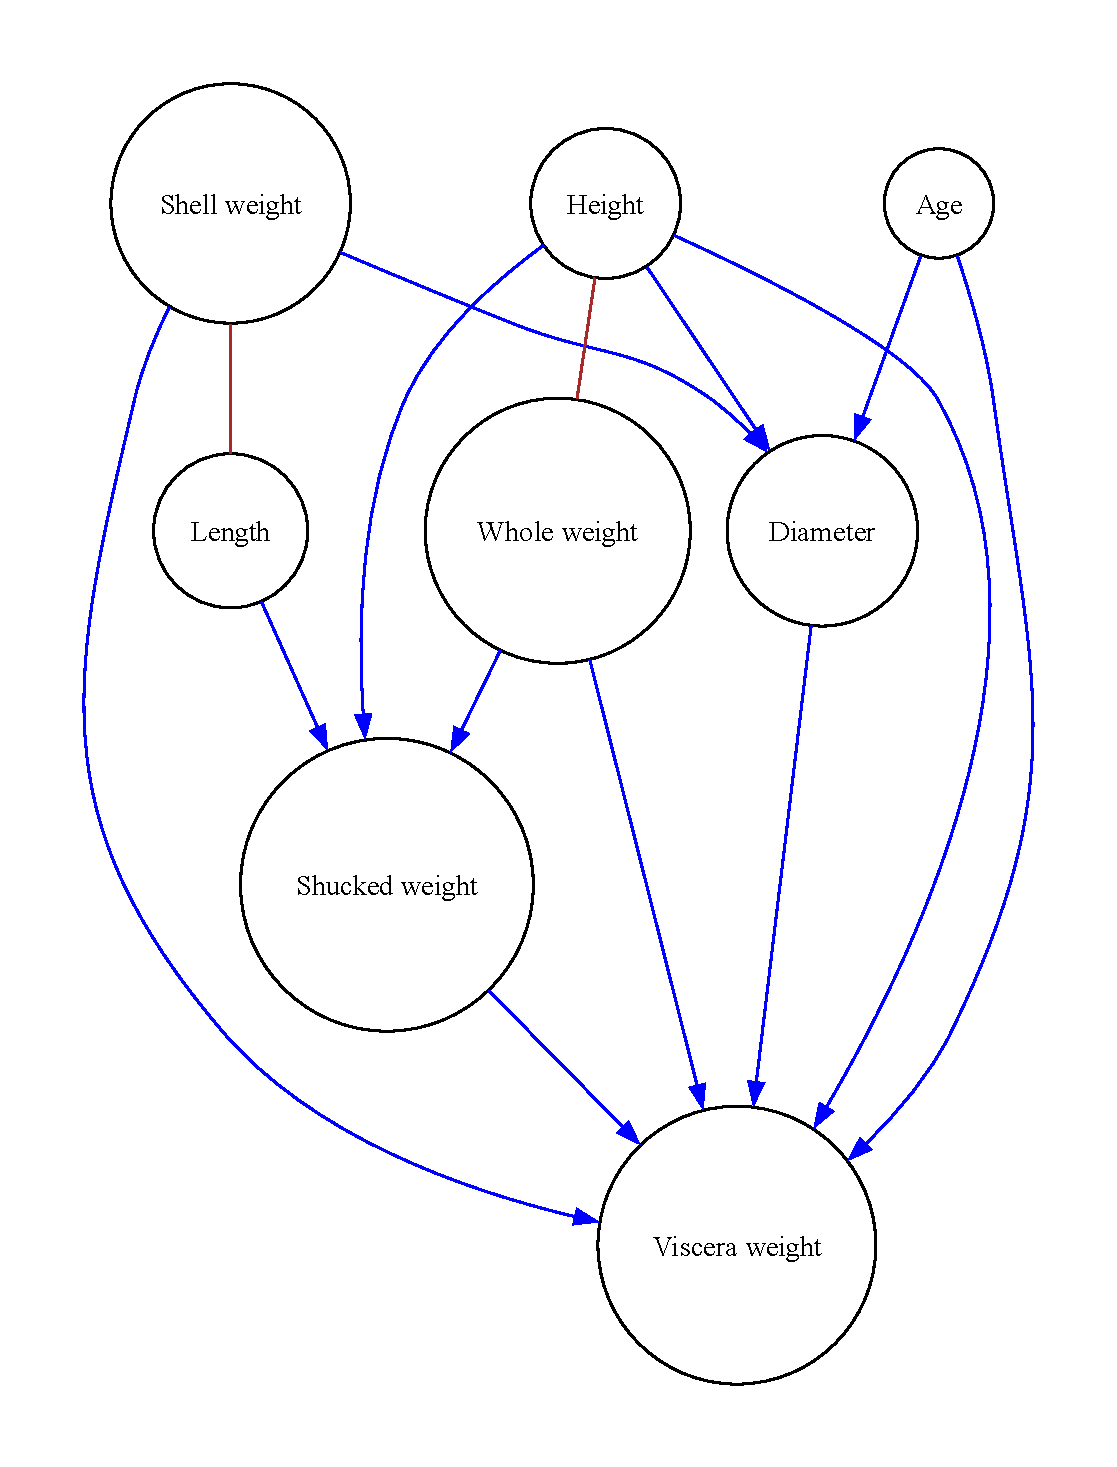
\includegraphics[width=\linewidth]{./demo_data/20241104_094220/Abalone/output_graph/initial_graph.pdf}
    \caption{Initial Graph}
\end{figure}

The above is the initial result graph produced by our algorithm.

The causal relationships among the variables reveal a complex interplay where Age influences Diameter and Viscera weight, suggesting that as an organism matures, its size and internal mass increase correspondingly. Length, a key physical dimension, impacts both Shell weight and Shucked weight, indicating that larger shells lead to greater overall body weight measured after processing. The interaction between Shell weight and Diameter further signifies that a heavier shell contributes to a broader overall size. Height also plays a significant role, affecting Diameter, Whole weight, Shucked weight, and Viscera weight, implying that greater height contributes to both physical dimensions and overall mass. Finally, Whole weight has cascading effects on Height, Shucked weight, and Viscera weight, demonstrating that overall body weight is a critical factor in determining a variety of physical and internal attributes, with Shucked weight being directly influenced by both Whole weight and Diameter. This demonstrates the interconnected nature of these variables in defining the growth and development of the organism.

\subsection{Revised Graph}

\begin{minipage}[t]{0.6\linewidth}
    
By using the method mentioned in the Section 4.4, we provide a revised graph pruned with Bootstrap and LLM suggestion.
Pruning results are as follows.
        
Bootstrap doesn't force or forbid any edges.
            
The following are force results given by LLM:
            
\begin{itemize}
            
\item \textbf{Age $\rightarrow$ Length}: Age is expected to causally influence length because abalones grow in size as they age, with older abalones typically being longer due to their prolonged growth periods.
                
\item \textbf{Age $\rightarrow$ Shell weight}: Shell weight is likely caused by age, as older abalones tend to have heavier shells due to continued growth and accumulation of shell material over time.
                
\item \textbf{Age $\rightarrow$ Height}: Height is expected to be causally related to age, as abalones increase in height as they mature, reflecting their overall growth.
                
\item \textbf{Age $\rightarrow$ Whole weight}: Whole weight is anticipated to be influenced by age, as older abalones usually have more biomass, leading to a greater total weight.
                
\item \textbf{Age $\rightarrow$ Shucked weight}: Shucked weight is likely affected by age because older abalones typically yield more edible flesh, resulting in a higher weight after the shell is removed.
                
\item \textbf{Length $\rightarrow$ Diameter}: Length and diameter are causally related as they both measure physical dimensions of the abalone. An increase in length generally correlates with an increase in diameter as the organism grows.
                
\item \textbf{Length $\rightarrow$ Height}: Length influences height; as abalones grow longer, they also typically grow taller, reflecting a consistent growth pattern in their morphology.
                
\item \textbf{Length $\rightarrow$ Whole weight}: Whole weight is expected to be caused by length, since longer abalones generally have more tissue and shell, leading to an increased total weight.
                
\item \textbf{Length $\rightarrow$ Viscera weight}: Viscera weight is likely influenced by length because larger abalones tend to have larger internal organs, resulting in greater viscera weight.
                
\item \textbf{Shell weight $\rightarrow$ Height}: Shell weight is causally related to height, as taller abalones usually possess thicker shells, contributing to increased shell weight.
                
\item \textbf{Shell weight $\rightarrow$ Whole weight}: Whole weight is expected to be influenced by shell weight, as a heavier shell adds to the overall mass of the abalone.
                
\item \textbf{Shell weight $\rightarrow$ Shucked weight}: Shucked weight is likely affected by shell weight since heavier shells typically indicate larger, more substantial abalones that yield more meat when shucked.
                
\item \textbf{Diameter $\rightarrow$ Whole weight}: Whole weight is anticipated to be influenced by diameter, as wider abalones usually have more mass, thereby increasing their total weight.
                
\item \textbf{Diameter $\rightarrow$ Shucked weight}: Shucked weight is likely influenced by diameter, since wider abalones often contain more edible tissue and therefore yield a greater amount of meat when processed.
                
\end{itemize}
            
The following are directions of remaining undirected edges determined by the LLM:
\begin{itemize}

\item \textbf{Length $\rightarrow$ Shell weight}: Length is likely a significant factor that directly influences shell weight because as abalones grow longer, their shells also tend to become heavier due to increased shell material and structural growth as the individual matures.

\item \textbf{Height $\rightarrow$ Whole weight}: Height contributes to the overall size of the abalone, and a greater height typically correlates with an increase in soft tissue and shell structure, leading to a higher whole weight as more biomass is accumulated.

\end{itemize}
            
This structured approach ensures a comprehensive and methodical analysis of the causal relationships within the dataset.
        
\vfill
\end{minipage}
\hfill
\begin{minipage}[t]{0.4\linewidth}
    \begin{figure}[H]
        \centering
        \vspace{-0.5cm}
        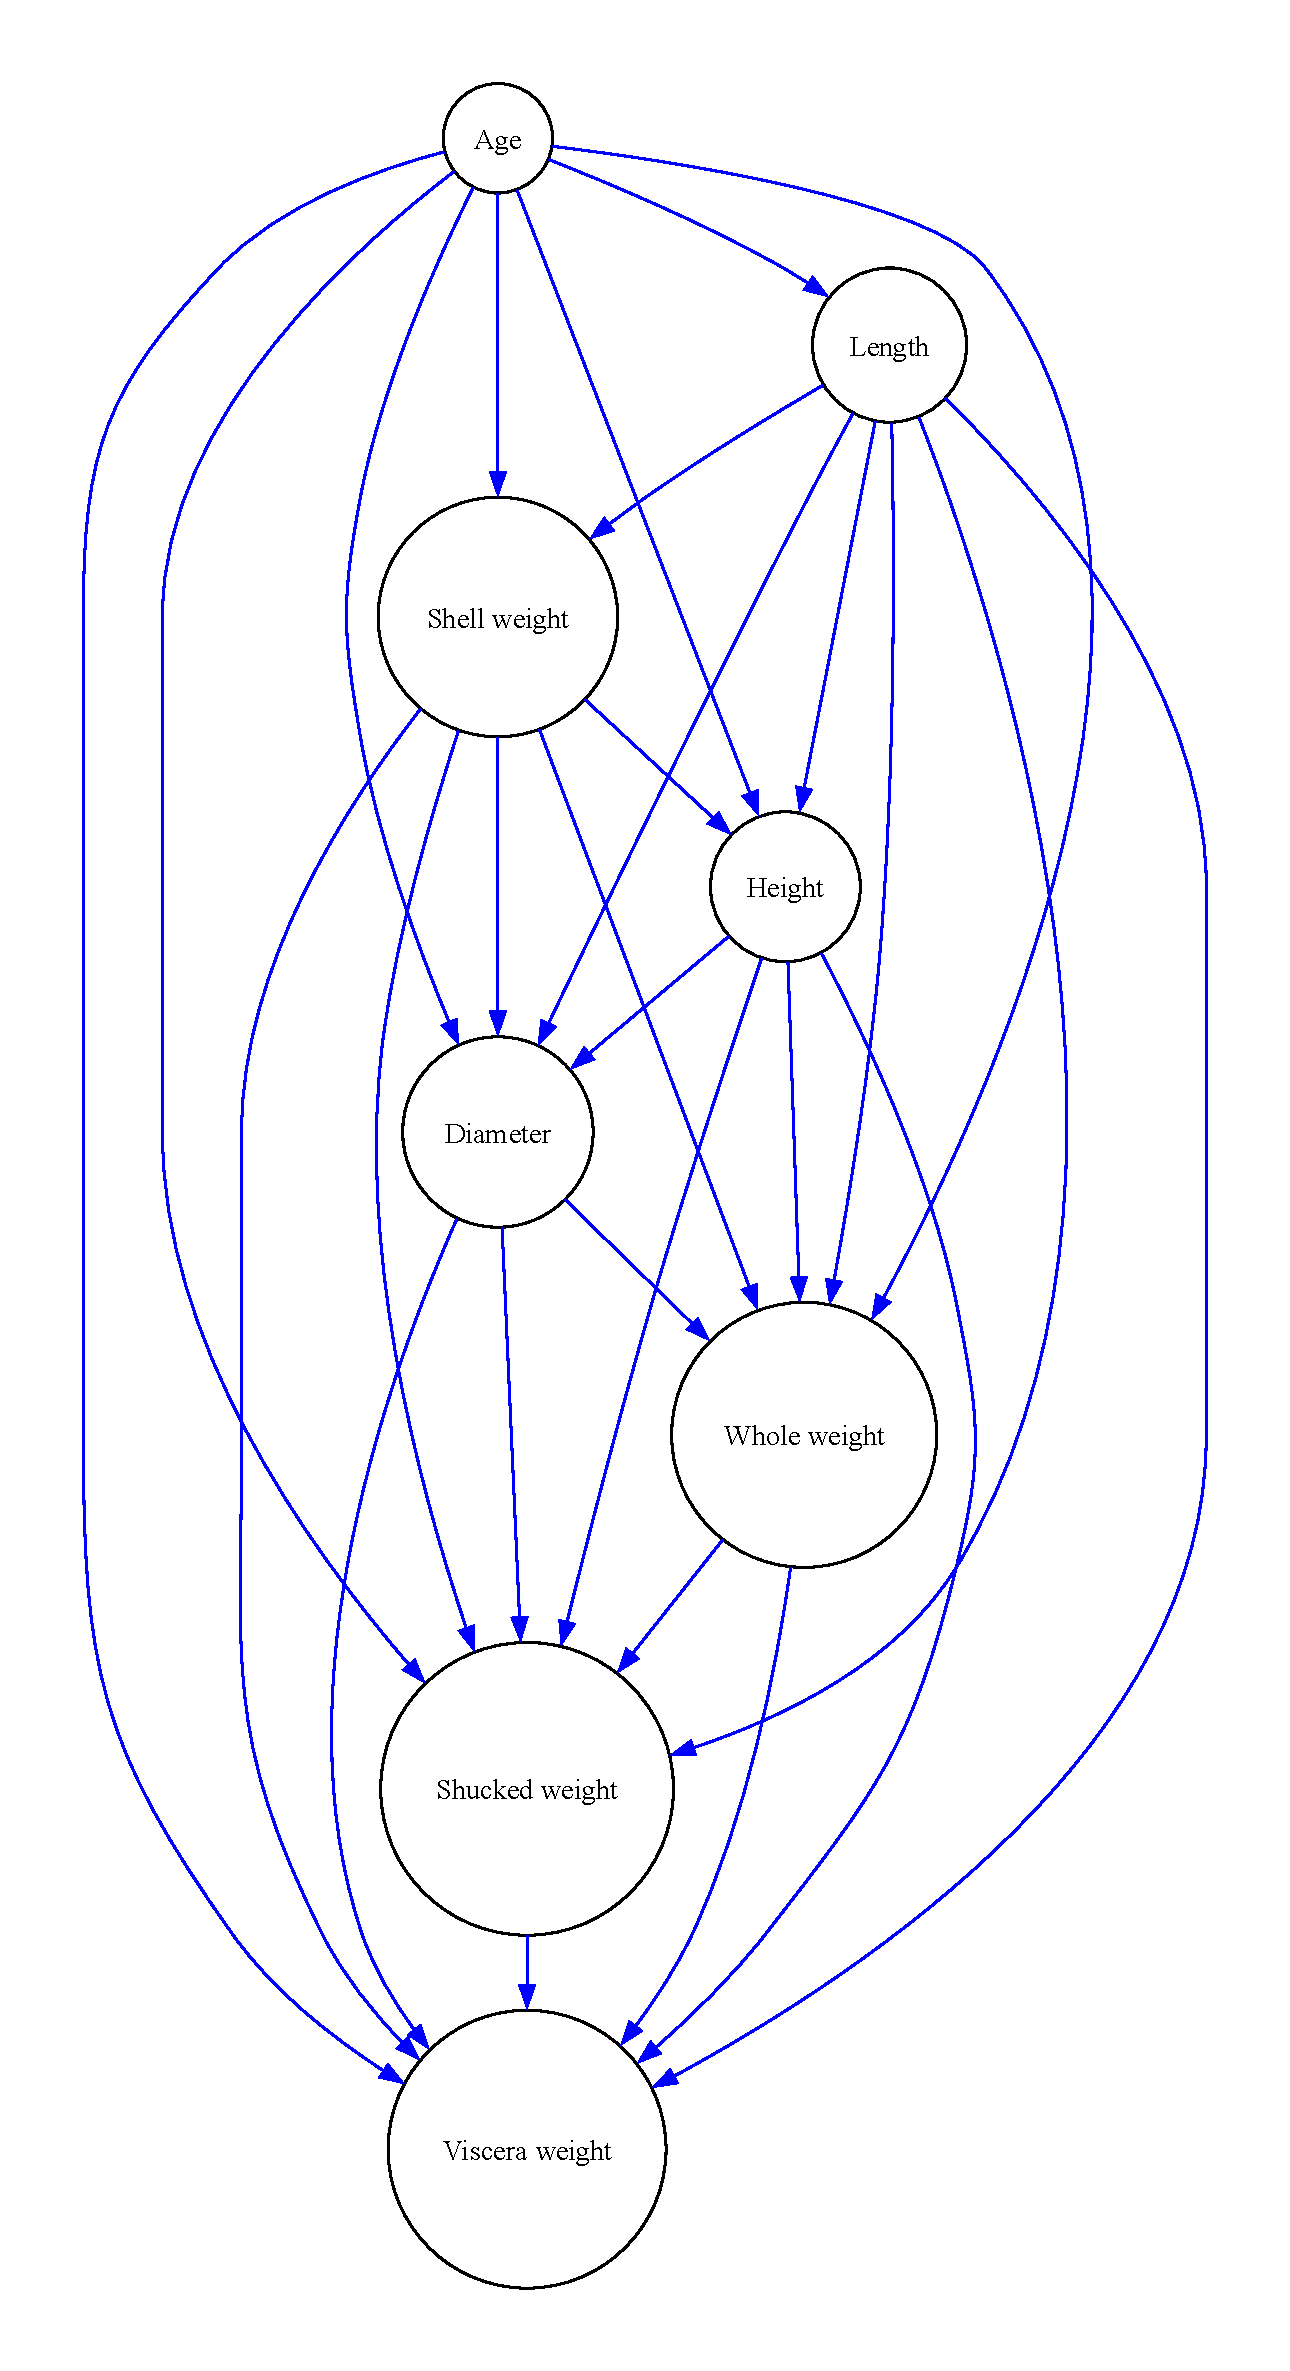
\includegraphics[width=\linewidth]{./demo_data/20241104_094220/Abalone/output_graph/revised_graph.pdf}
        \caption{\label{fig:corr}Revised Graph}
    \end{figure}
\end{minipage}

\subsection{Graph Reliability Analysis}

\begin{figure}[H]
    \centering

    \begin{subfigure}{0.32\textwidth}
        \centering
        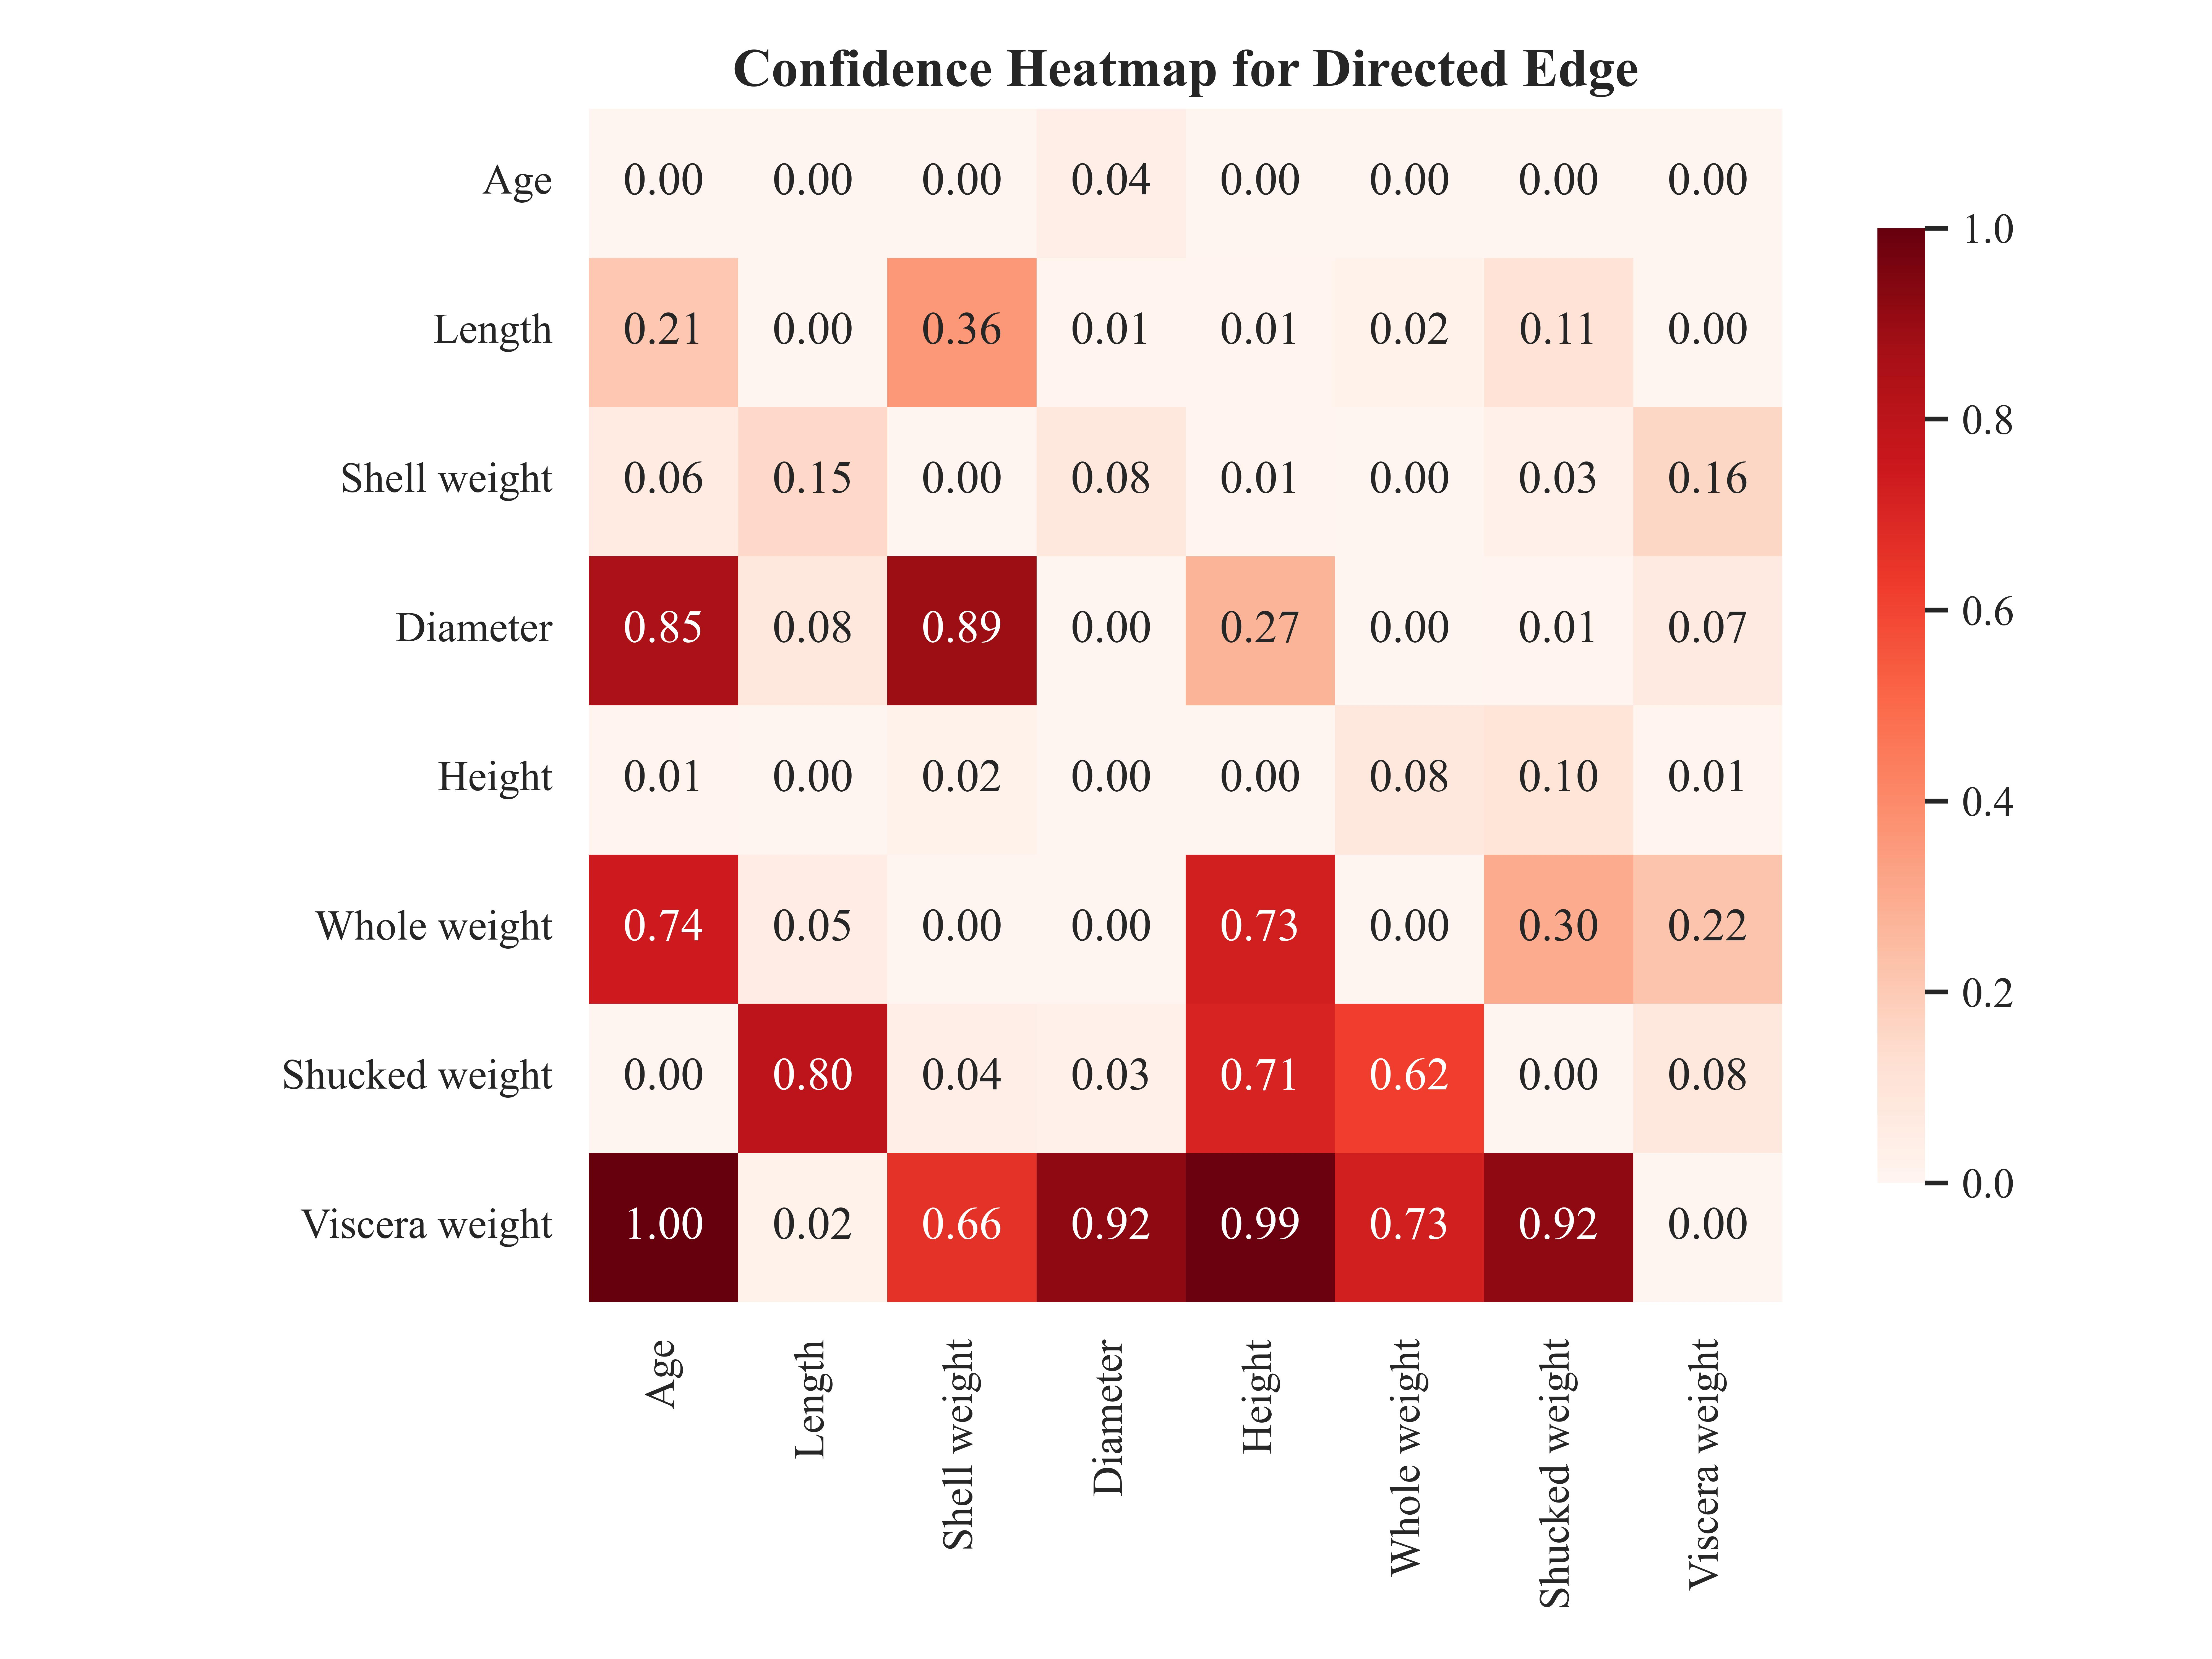
\includegraphics[width=\linewidth]{./demo_data/20241104_094220/Abalone/output_graph/certain_edges_confidence_heatmap.jpg}
        \caption{Directed Edge Edge}
    \end{subfigure}
    \begin{subfigure}{0.32\textwidth}
        \centering
        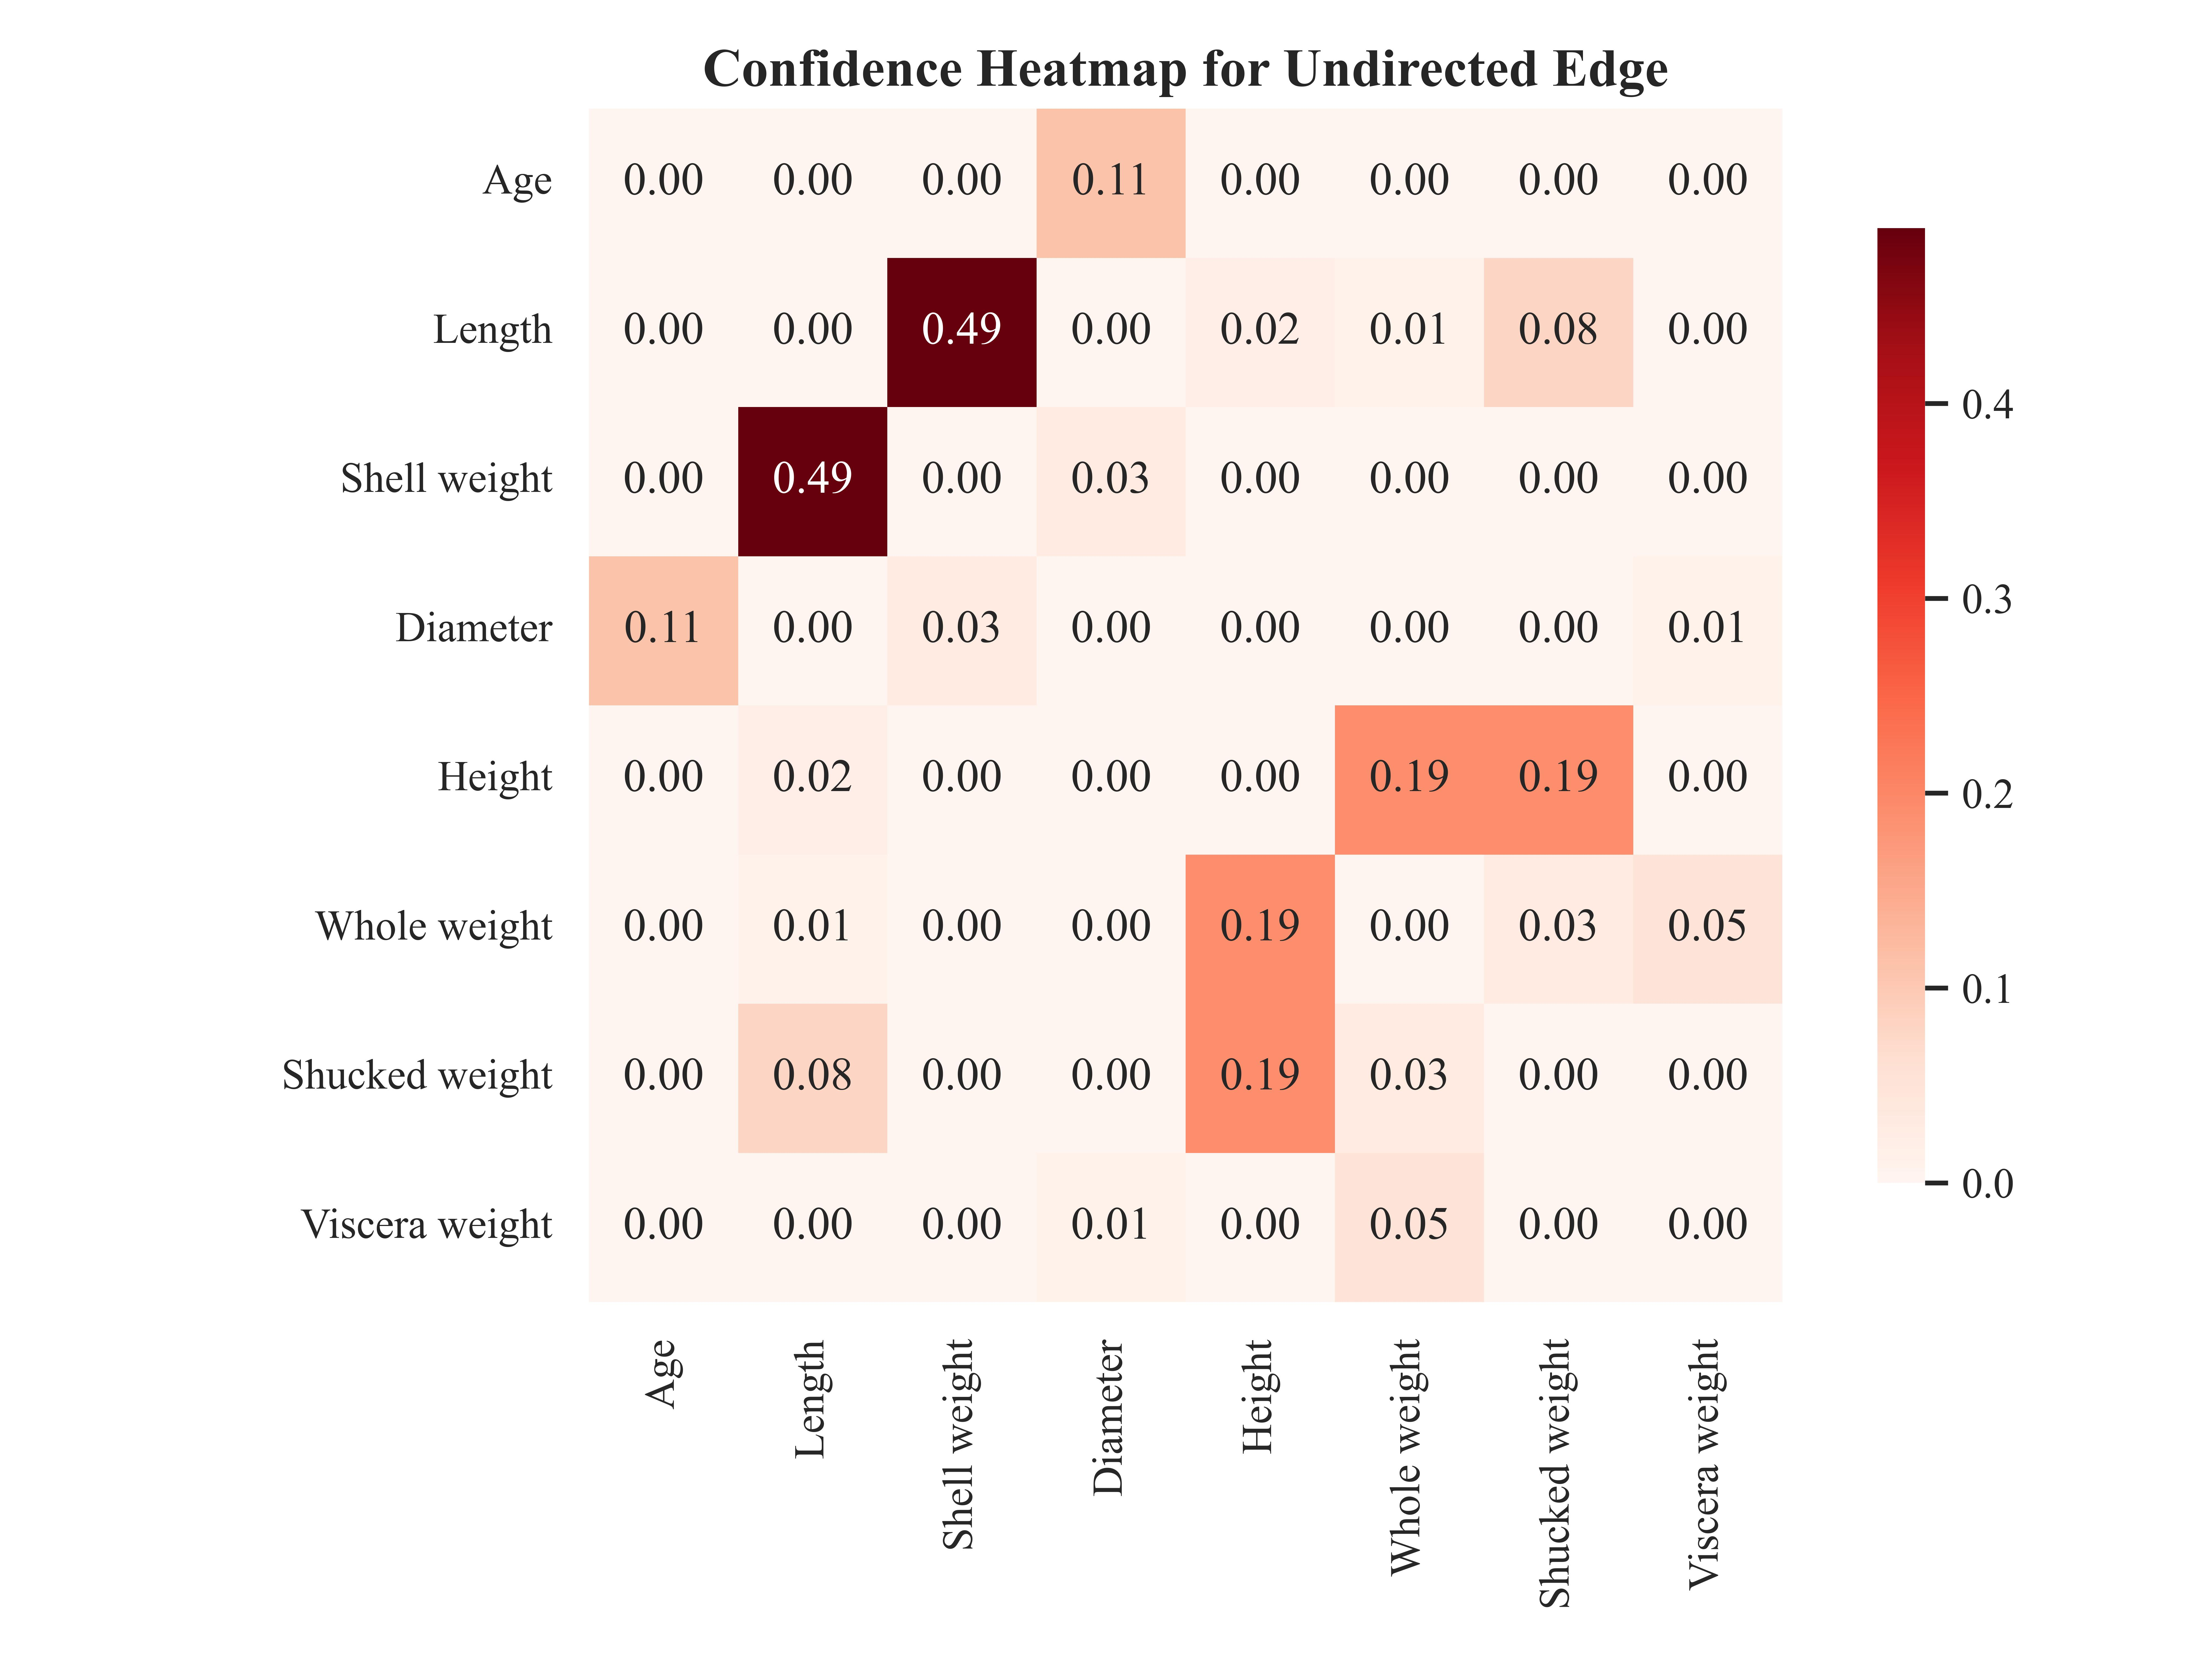
\includegraphics[width=\linewidth]{./demo_data/20241104_094220/Abalone/output_graph/uncertain_edges_confidence_heatmap.jpg}
        \caption{Undirected Edge Edge}
    \end{subfigure}
    \begin{subfigure}{0.32\textwidth}
        \centering
        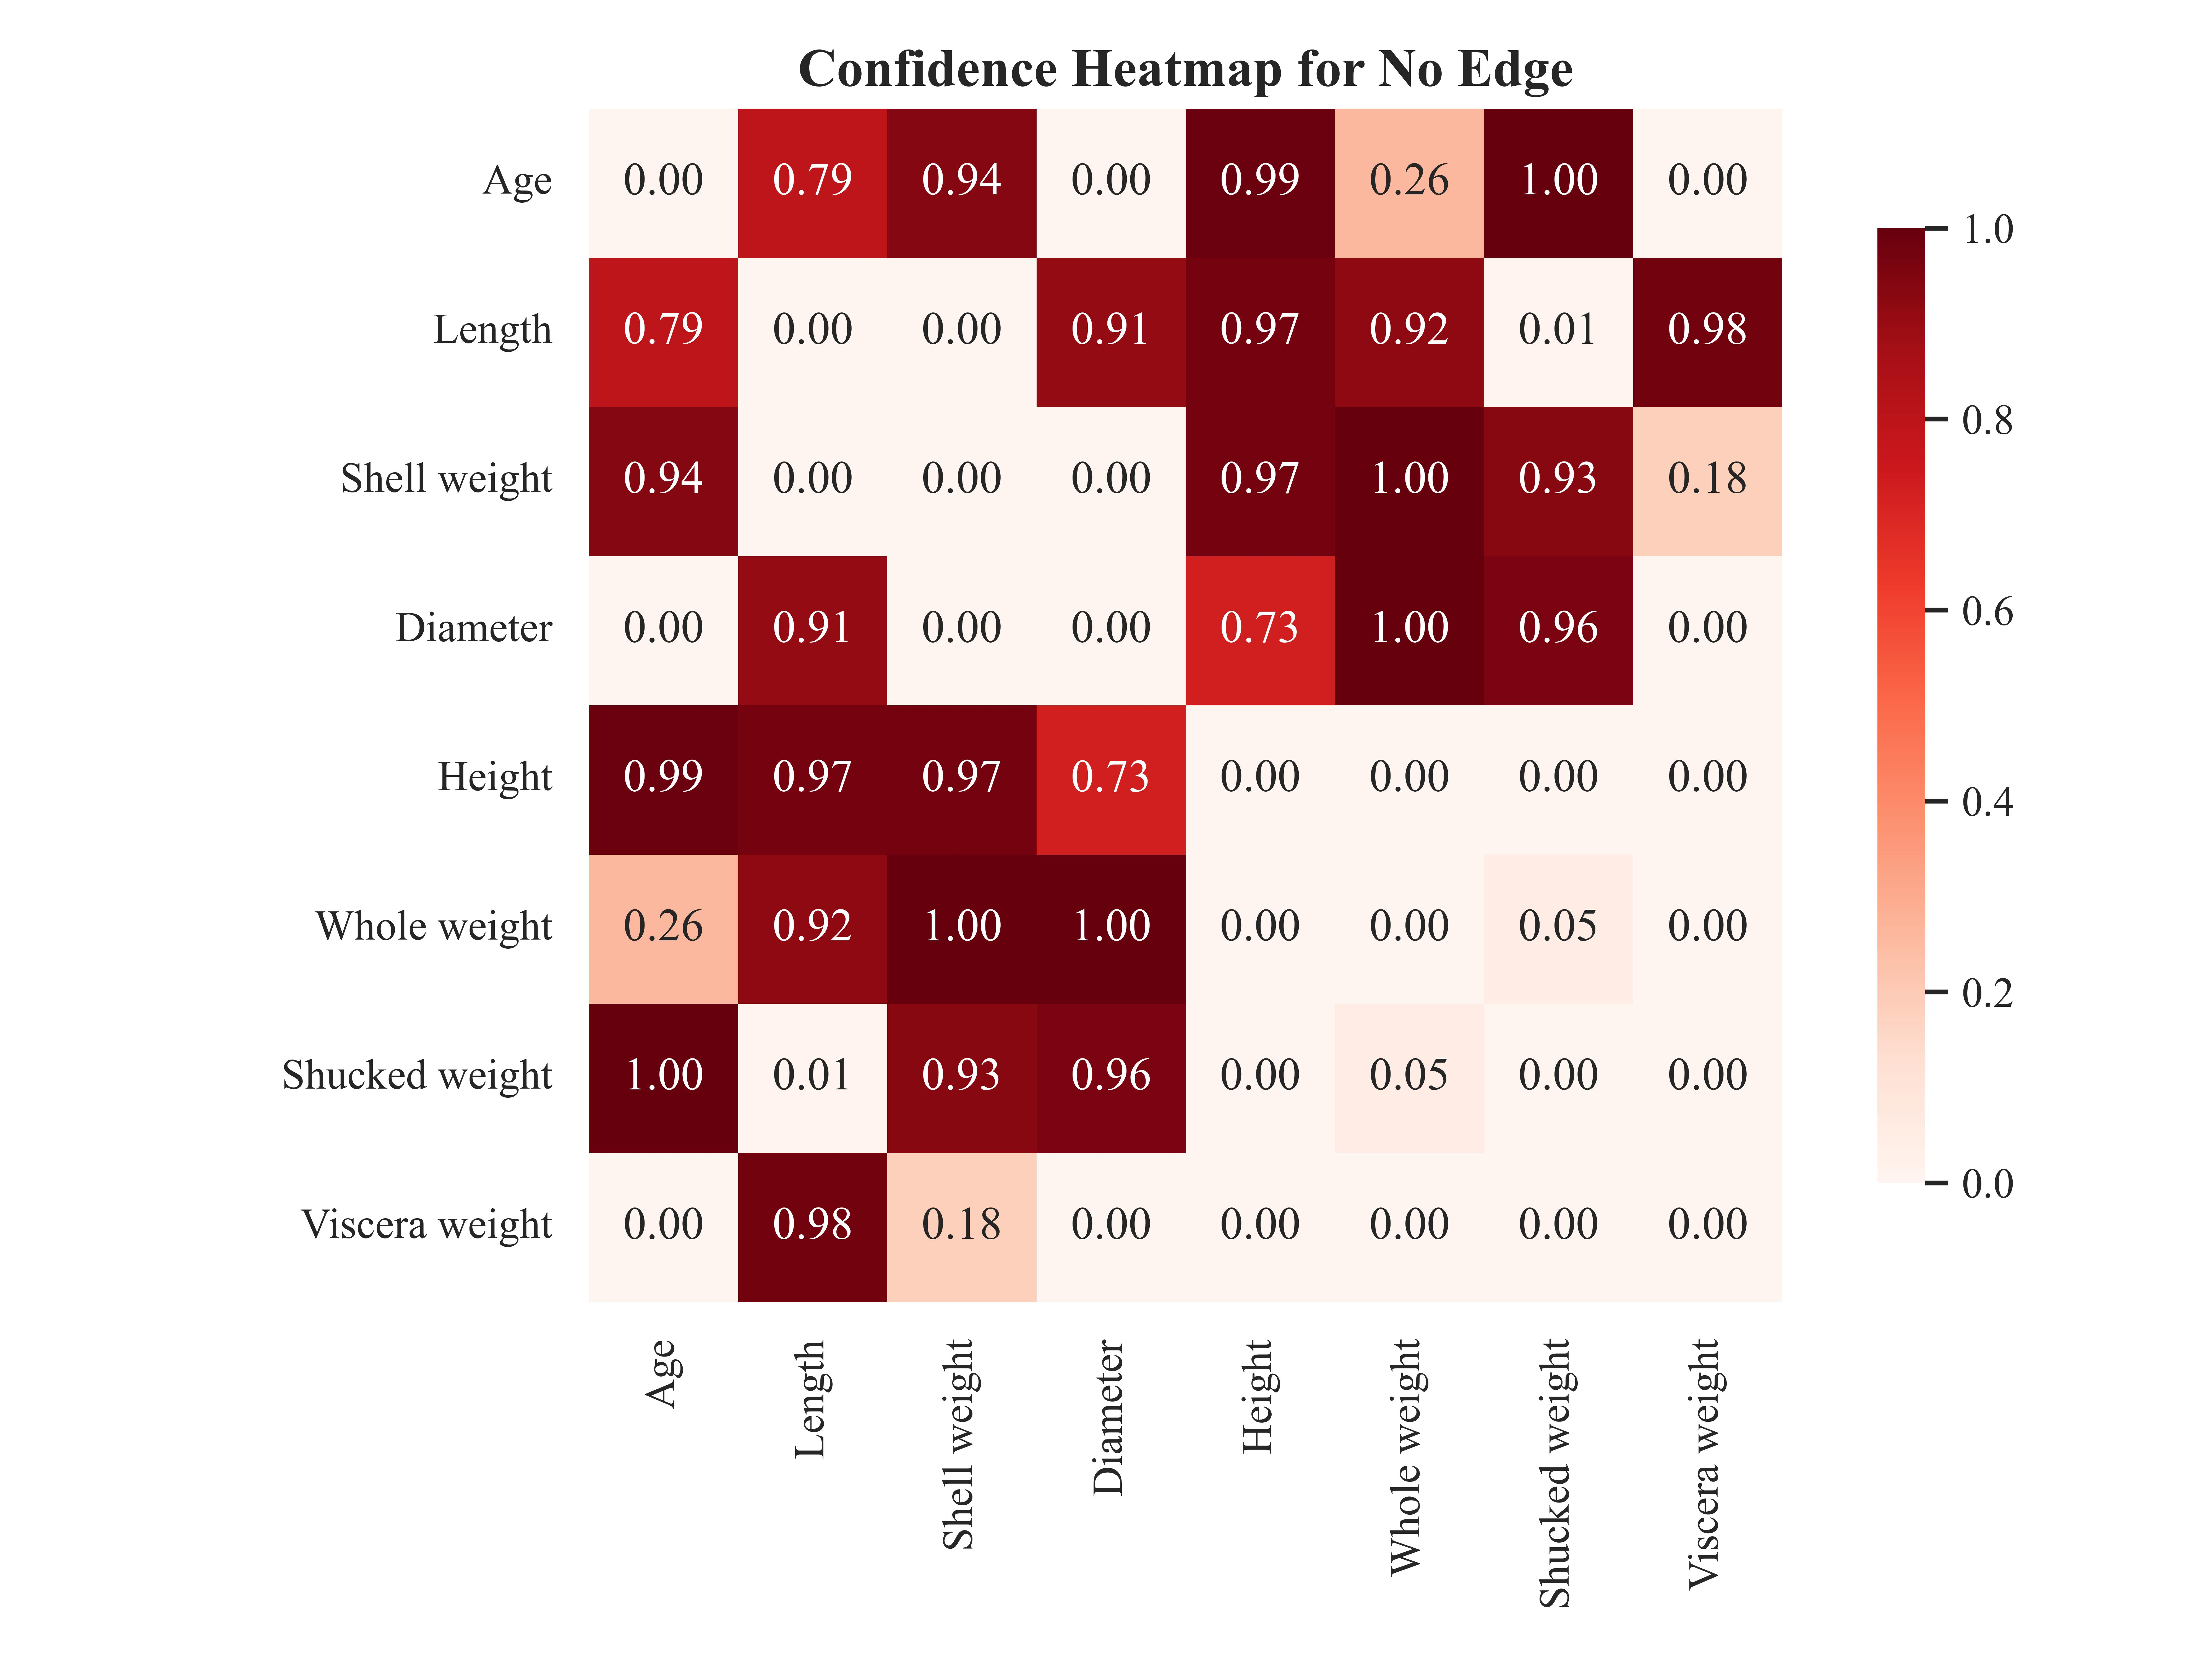
\includegraphics[width=\linewidth]{./demo_data/20241104_094220/Abalone/output_graph/non_existence_confidence_heatmap.jpg}
        \caption{No Edge Edge}
    \end{subfigure}
    \caption{Confidence Heatmap of Different Edges}
\end{figure}        

The above heatmaps show the confidence probability we have on different kinds of edges, including directed edge ($\rightarrow$), undirected edge ($-$), No Edge, and probability of no edge. The heatmap of bi-edges is not shown because probabilities of all edges are 0. Based on the confidence probability heatmap and background knowledge, we can analyze the reliability of our graph.

From the statistics perspective, we have high confidence to believe that the edges \textbf{Whole weight $\rightarrow$ Height (0.73)}, \textbf{Whole weight $\rightarrow$ Shucked weight (0.3)}, and \textbf{Length $\rightarrow$ Shell weight (0.36)} exist, as these edges have relatively high bootstrap probabilities indicative of a stronger causal relationship. Conversely, we have low confidence in the edges \textbf{Age $\rightarrow$ Diameter (0.04)} and \textbf{Age $\rightarrow$ Viscera weight (0.0)}, suggesting they are unlikely to represent true causal relationships.

However, based on expert knowledge, we know that certain edges are highly plausible due to biological reality, such as the relationships between \textbf{Age} and size metrics like \textbf{Length, Diameter, and Height}, which are established in growth patterns of abalones as they mature. Additionally, the strong likelihood that \textbf{Shell weight contributes to Whole weight} correlates with our understanding of shell structure and overall biomass. Edges such as \textbf{Height $\rightarrow$ Viscera weight (0.01)} and \textbf{Diameter $\rightarrow$ Viscera weight (0.07)} also seem less causally substantial given the biological context.

Therefore, the result of this causal graph is not entirely reliable, as there is a significant discrepancy between the statistical confidence and the expert biological insights regarding the causal relationships, particularly concerning the age-related edges and certain other connections that are less supported by domain knowledge.

\end{document}